\documentclass{article} 
\usepackage[fleqn]{amsmath}
\usepackage{graphicx}
\usepackage{mathrsfs}
\usepackage{color}
\usepackage{amssymb}
\usepackage{amsfonts,amssymb}
\usepackage{algorithm}
\usepackage{algorithmic}
\usepackage{array}
\usepackage{latexsym}
\usepackage{hyperref}



\title{\normalsize
CS410: Artificial Intelligence 2021 Fall\\
Homework 3: Local Search \& Adversarial Search \& MDP\\
Due date: 23:59:59 (GMT +08:00), November 6 2021}
\author{}
\date{}

\begin{document} 
\maketitle

\begin{enumerate}
    \item \textbf{Local Search}.
    The traveling salesman problem (TSP) is the problem of finding the shortest route to visit a set of cities exactly once and return to the starting city. 
Describe how to use genetic algorithm for TSP. Propose a state representation, the corresponding crossover and mutation, and the fitness function.\\
~\par
    \textbf{Solution:}
    \begin{enumerate}
        \item \textbf{State:}$S=\{s_1,s_2,s_3\dots s_n\}$ is a rotation of the $[n]$ and represents the route. The salesman travels the city $s_i$ at the $i^{th}$ time and returns to city $s_1$.
        \item \textbf{Crossover:}Given two state $S^{1},S^{2}$, we run the crossover algorithm to get two new states $\overline{S}^{1},\overline{S}^{2}.$
        \begin{enumerate}
            \item Assume $S^{1}=\{s_1^1,\dots s_n^1\},S^{2}=\{s_1^2,\dots s_n^2\}$, we generate two new temporary states\\ $S^{1'}=\{s_1^1,\dots s_{\lfloor \frac{n}{2}\rfloor}^1,s_{\lfloor \frac{n}{2}\rfloor+1}^2,\dots s_n^2\}$ \\$S^{2'}=\{s_1^2,\dots s_{\lfloor \frac{n}{2}\rfloor}^2,s_{\lfloor \frac{n}{2}\rfloor+1}^1,\dots s_n^1\}$.
            \item There must be repetitive city in $S^{1'}$. Assume $\exists p<=\lfloor \frac{n}{2}\rfloor, q>=\lfloor \frac{n}{2}\rfloor+1$ satisfying $S^{1'}[p]=S^{1'}[q]$, modify the $S^{1'}$ that $S^{1'}[p]=S^{2}[p]$. Repeat this operation until there is no repetitive elements in $S^{1'}$, then we get the $\overline{S}^{1}$.
            \item Also applying the same methods on $S^{2'}$ and get the $\overline{S}^{2}$.
        \end{enumerate}
        \item \textbf{Mutation:} For a given state $S$, we randomly choose 2 elements $1\le i<j\le n$ that exchange the $s_i, s_j$ in $S$ and get the new state.
        \item \textbf{Fitness Function:}Let $S=\{s_1,s_2,s_3\dots s_n\}$, and we define the fitness function $f$ that
        \begin{equation}
            f(S)=\frac{1}{\sum_{i=1}^{n}d(s_i,s_{i+1})}~~~with~~~s_{n+1}:=s_1
        \end{equation}
    \end{enumerate}
    
    \item \textbf{Game Tree}.
Prove that with a positive linear transformation of leaf values (i.e., transforming a value $x$ to $ax + b$ where $a > 0$), the choice of move remains unchanged in a game tree, even when there are chance nodes.\\
    \begin{figure}[h]
        \centering
        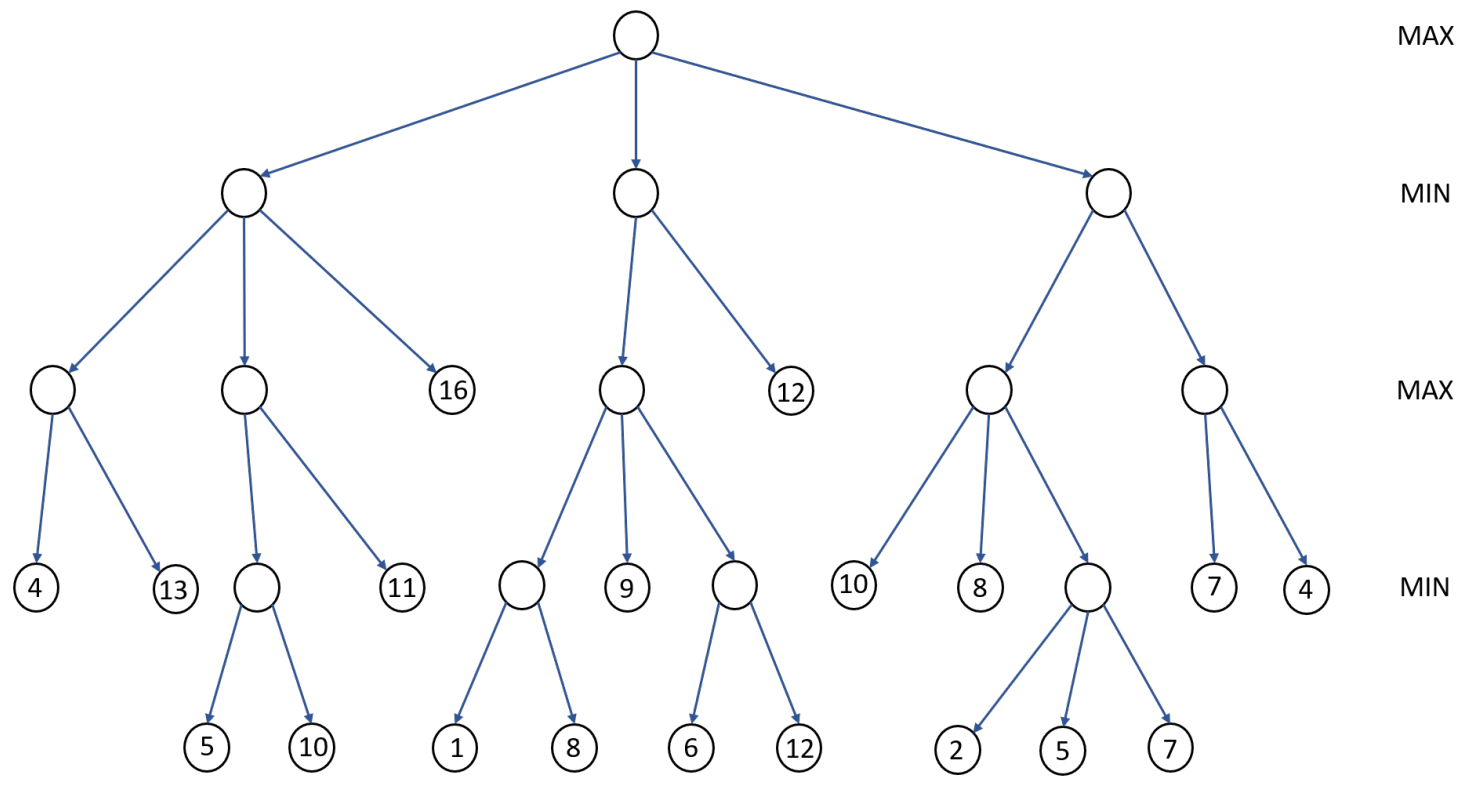
\includegraphics[width=12cm]{figs/fig_p3.png}
        \label{fig:p3}
        \caption{Problem 3.}
    \end{figure}
\par
\textbf{Solution:}\\
Let $f$ be the positive linear transformation that $f(x)=a*x+b$. We prove it step by step.
\begin{enumerate}
    \item $x_1\le x_2\Leftrightarrow f(x_1)\le f(x_2)$.That's because 
    \begin{equation}
        x_1\le x_2\Leftrightarrow a*x_1\le a*x_2\Leftrightarrow f(x_1)\le f(x_2)~~~with~~~a>0
    \end{equation}
    \item From (a) we know
    \begin{equation}
    \begin{aligned}
        \mathop{\arg\max}\limits_{x}x=\mathop{\arg\max}\limits_{x}f(x)\\
        \mathop{\arg\min}\limits_{x}x=\mathop{\arg\min}\limits_{x}f(x)
    \end{aligned}
    \end{equation}
    So for all the max and min points $x$,
    \begin{equation}
    \begin{aligned}
         value(x)=\mathop{\arg\max}\limits_{y\in children(x)}=\mathop{\arg\max}\limits_{y\in children(x)}f(y)=f(x)\\
         value(x)=\mathop{\arg\min}\limits_{y\in children(x)}=\mathop{\arg\min}\limits_{y\in children(x)}f(y)=f(x)
    \end{aligned}
    \end{equation}
    \item For any probability sequenses $\{\alpha_1\dots\alpha_n\}$ with $\sum\limits_{i=1}^{n}\alpha_i=1$, and a value sequense $X=\{x_1\dots x_n\}$. We have 
    \begin{equation}
        \begin{aligned}
        &f(\sum_{i=1}^{n}\alpha_i*x_i)\\
        =&a*\sum_{i=1}^{n}\alpha_i**x_i+b\\
        =&\sum_{i=1}^{n}\alpha_i*(a*x_i)+b*\sum_{i=1}^{n}\alpha_i\\
        =&\sum_{i=1}^{n}\alpha_i*[(a*x_i)+b]\\
        =&\sum_{i=1}^{n}\alpha_i*f(x_i)
        \end{aligned}
    \end{equation}
    \item So for the chance nodes $x$, we also have $value(x)=f(x)$. 
\end{enumerate}
From (a) to (d) we can conclude that the choice of move remains unchanged.
    \item \textbf{Alpha-Beta Pruning}.
    Consider the above game tree.
    \begin{enumerate}
        \item	Compute the minimax value for each node using Minimax algorithm.
        \item	Prune the game tree using Alpha-Beta pruning algorithm. Provide the final alpha and beta values computed at the root, each internal node visited, and at the top of pruned branches. Provide the pruned branches. Assume child nodes are visited from left to right.
    \end{enumerate}
    \textbf{Solution:}\\
    Please refer to the following figures~\ref{Solution3}
    \begin{figure}[h]
    	    \centering
    	    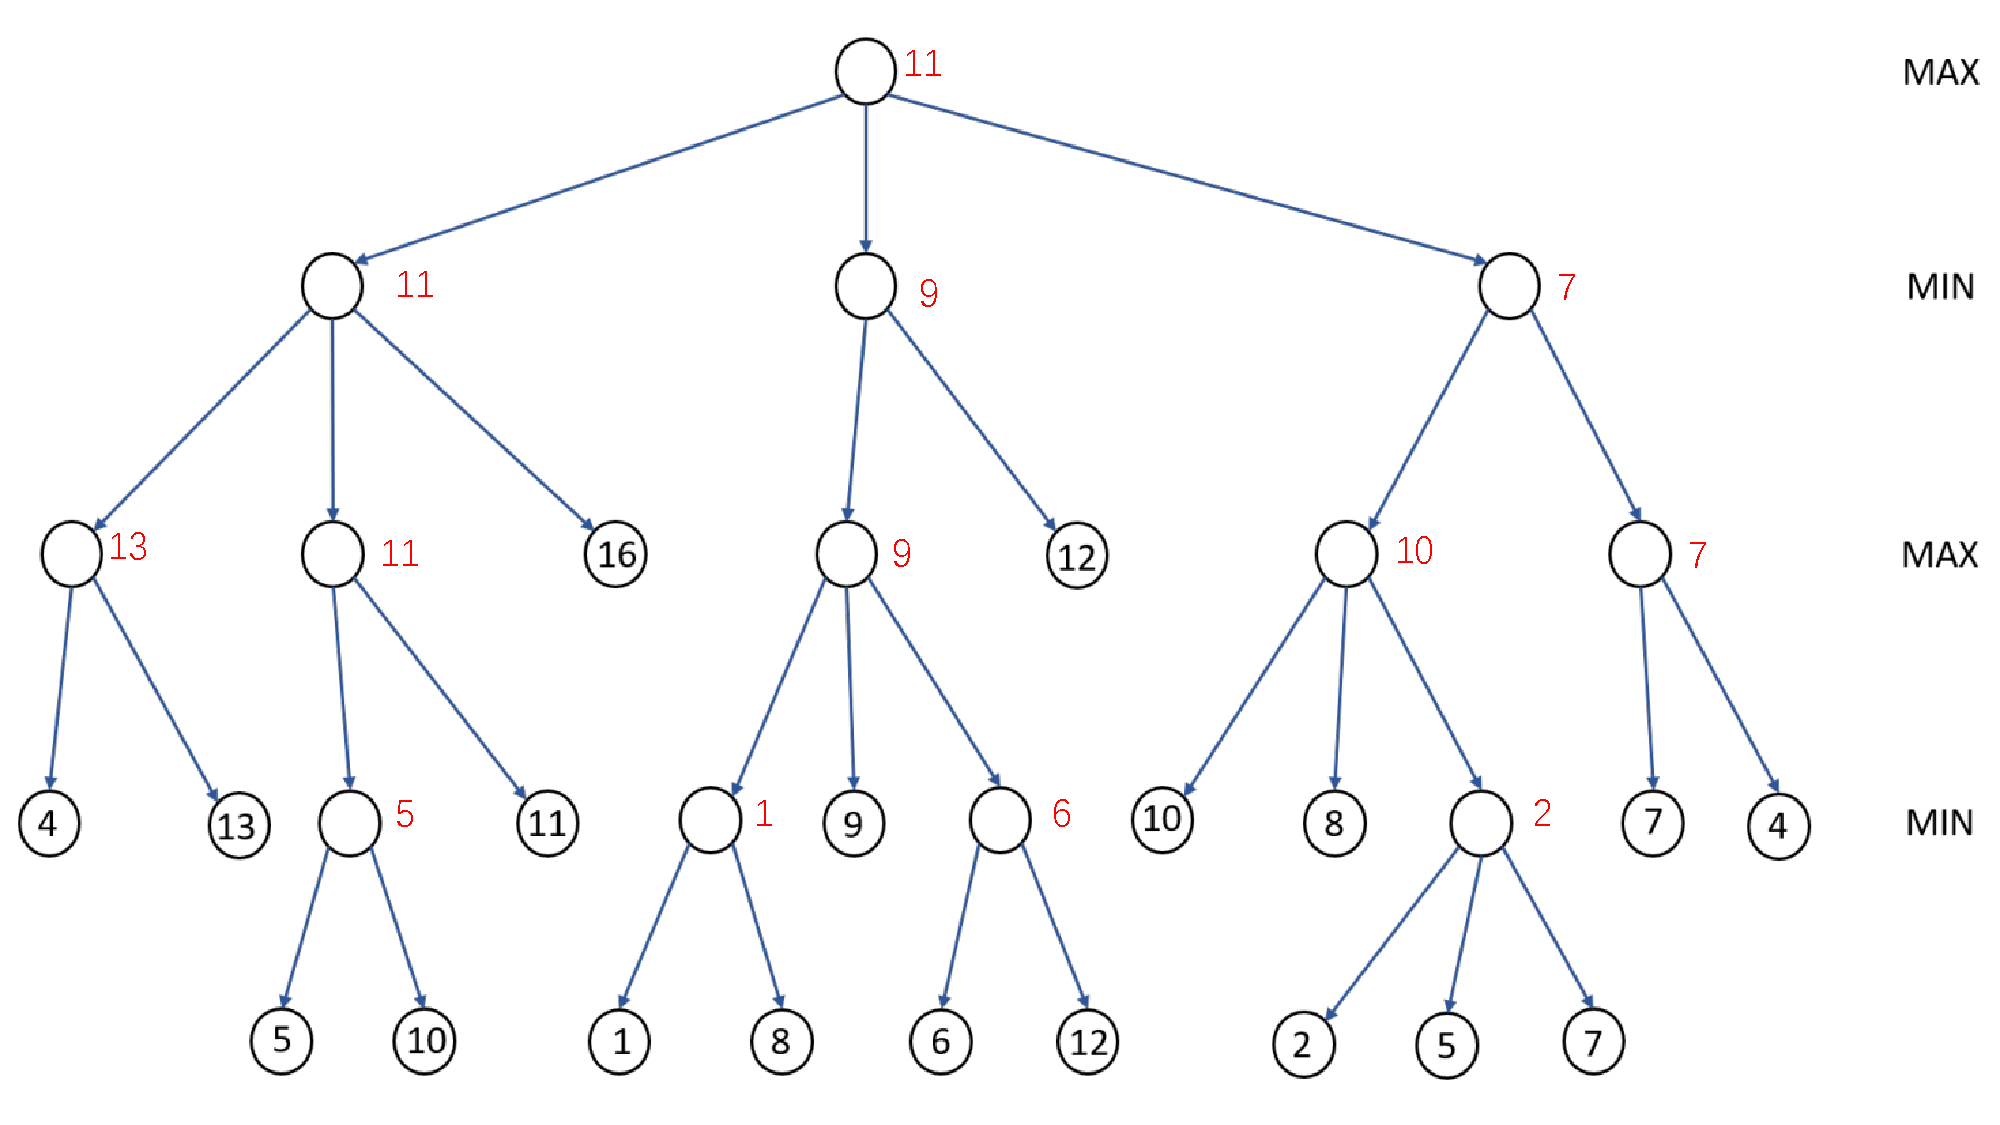
\includegraphics[width=1\textwidth]{figs/problem3.1.pdf}
    	    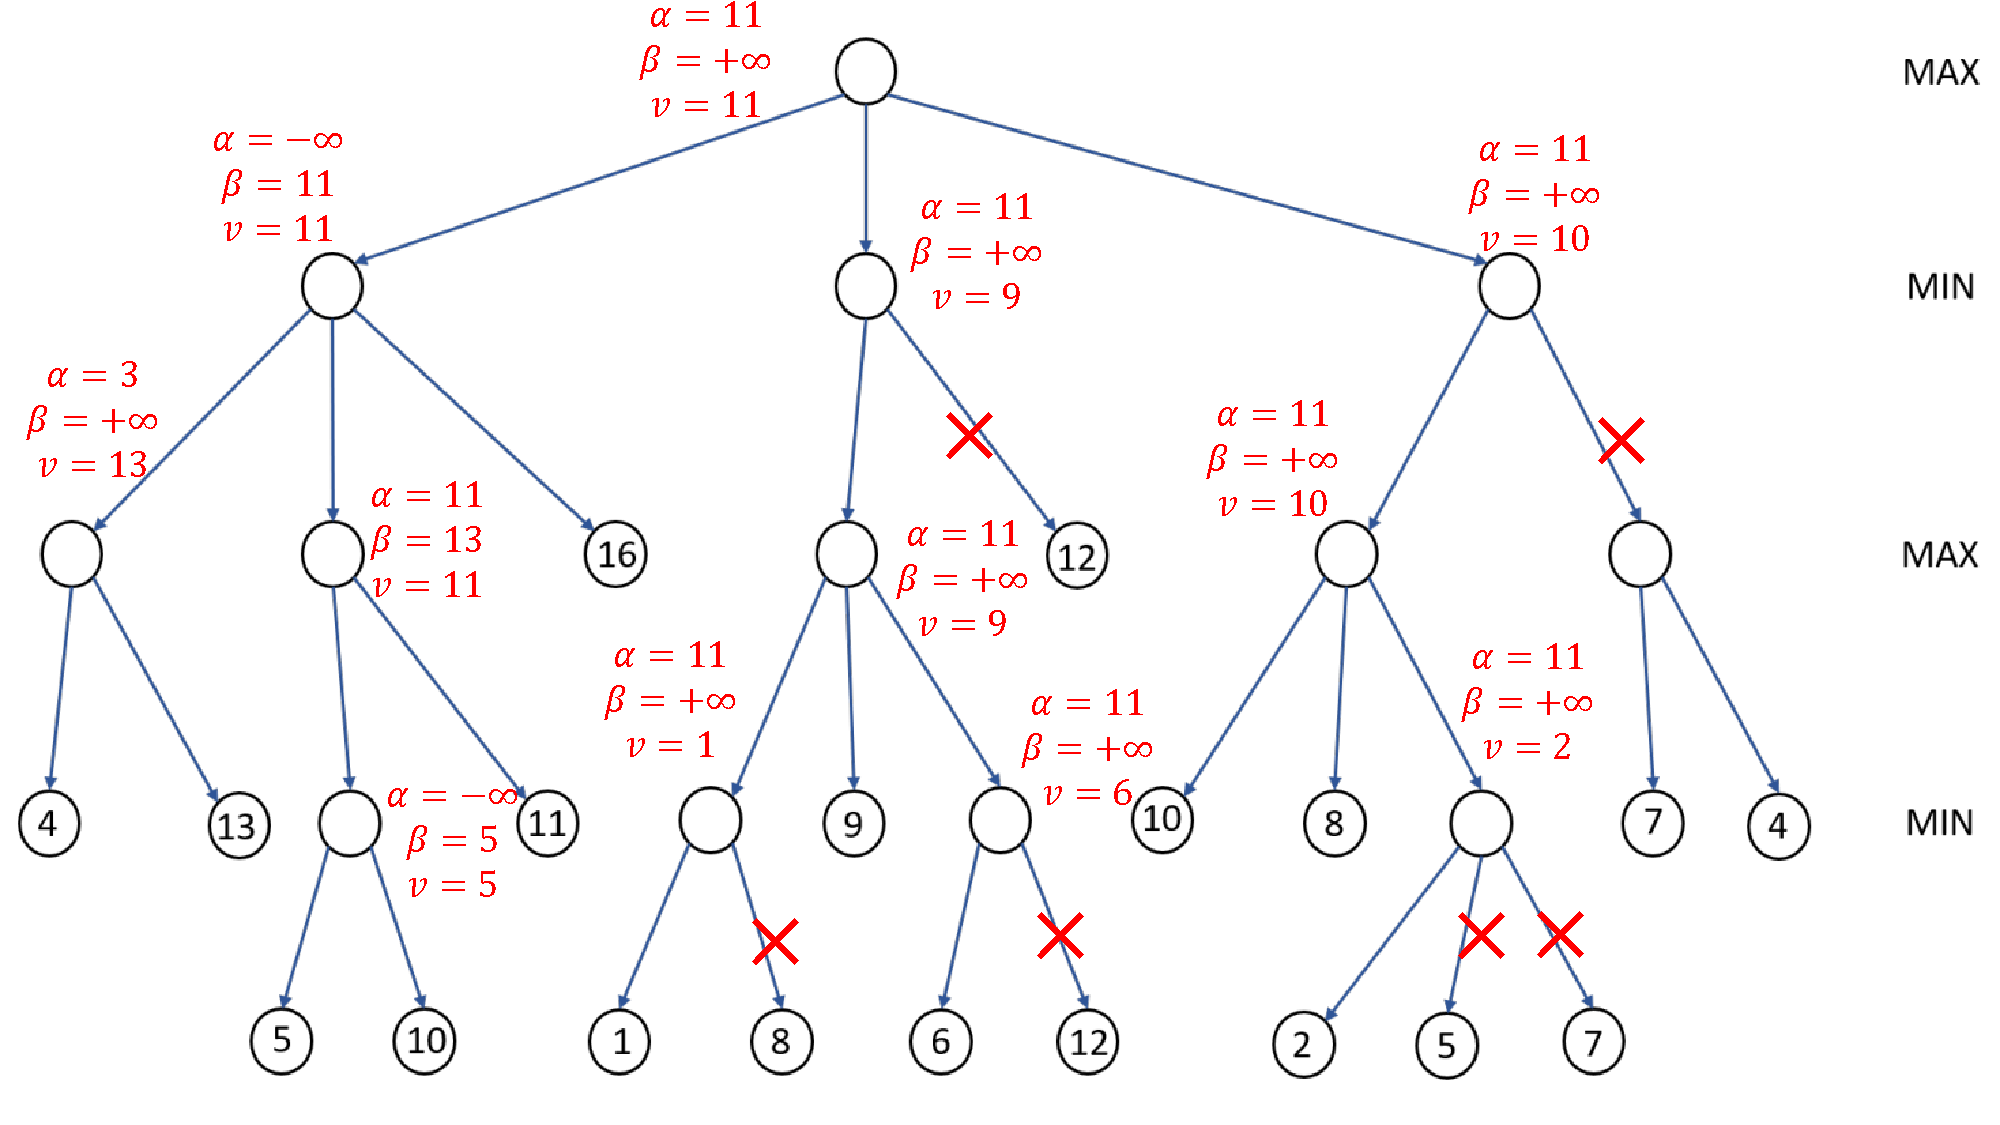
\includegraphics[width=1\textwidth]{figs/problem3.2.pdf}
    	    \caption{Solution 3}
    	    \label{Solution3}
    \end{figure}
    \item \textbf{Racing Problem}.
    	Consider the racing problem in Page 17, Lecture 6.
    	
    	\begin{figure}[h]
    	    \centering
    	    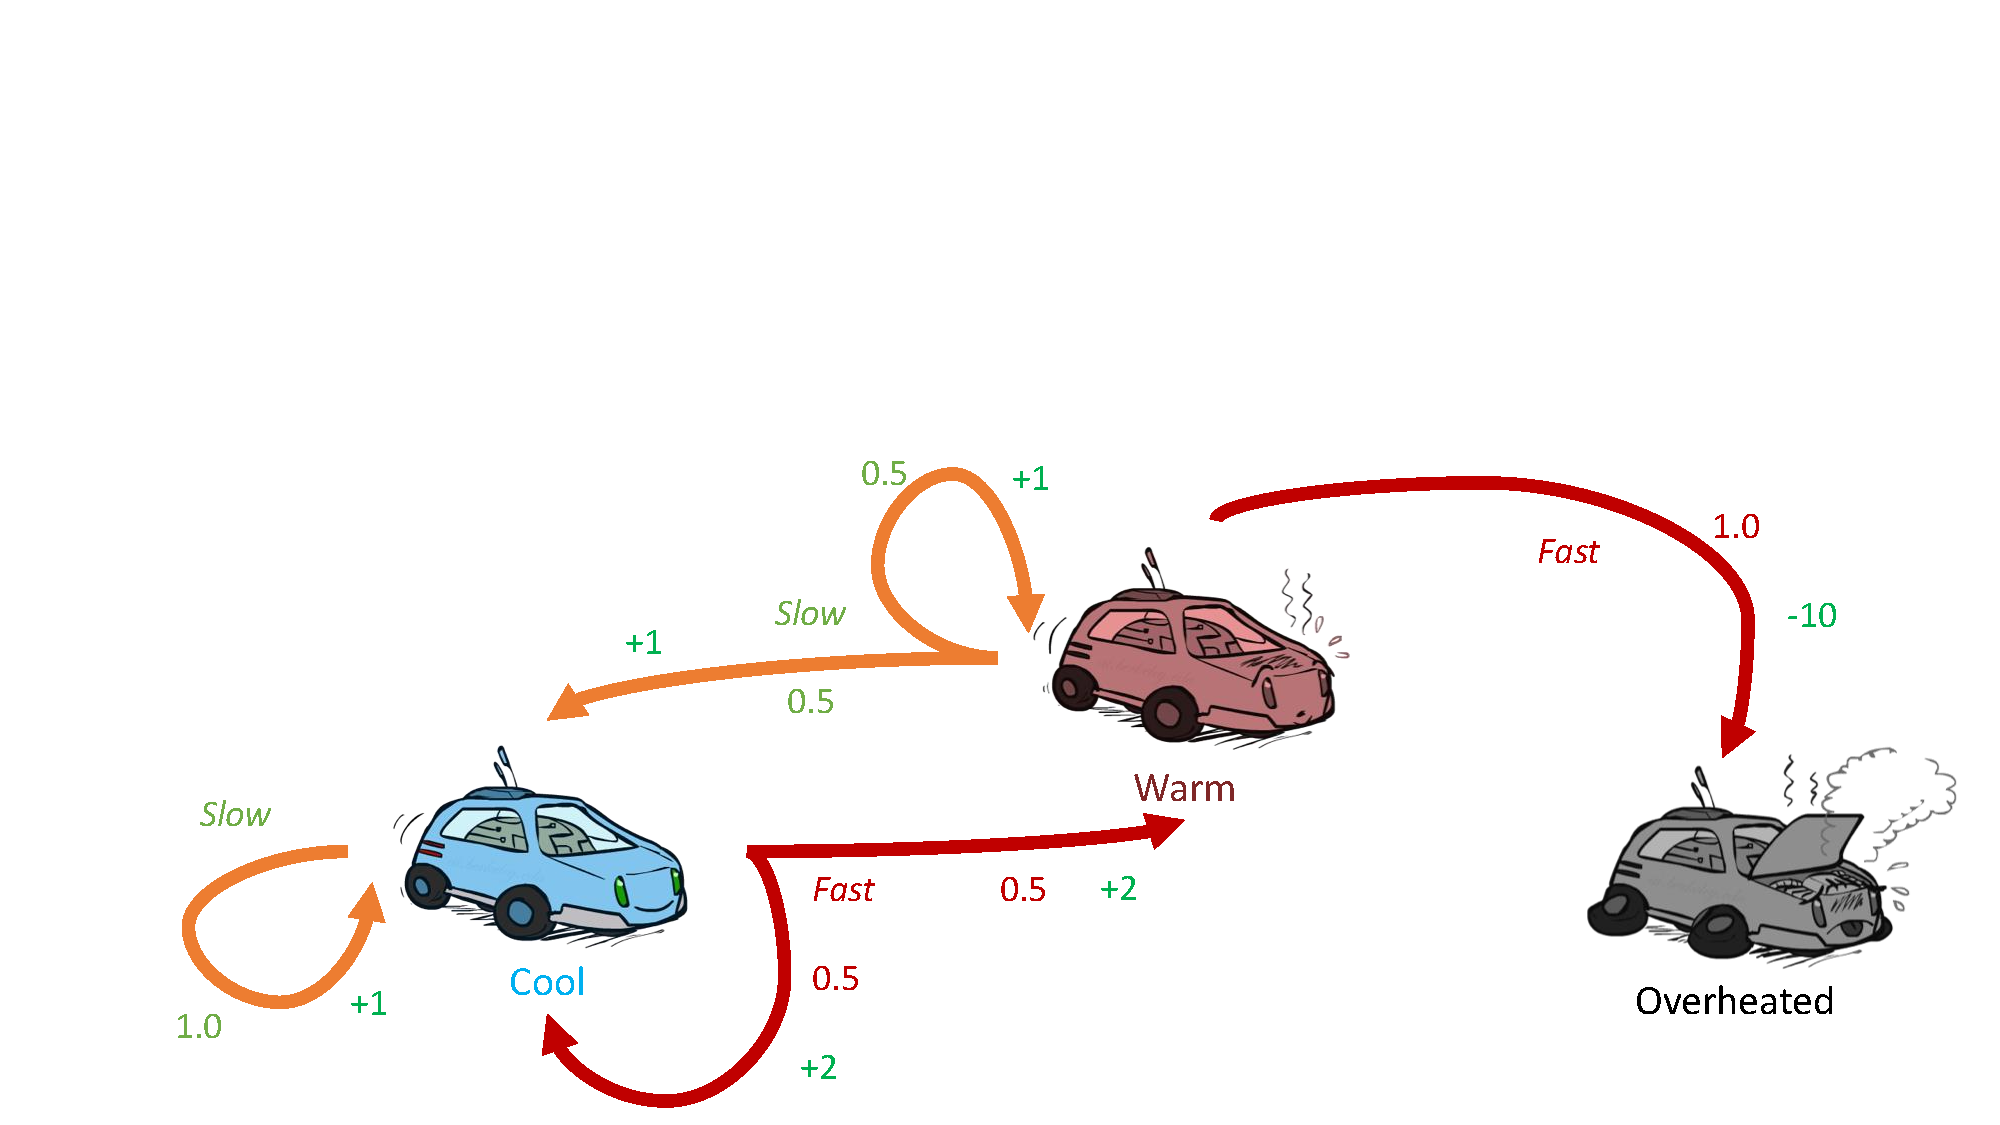
\includegraphics[width=12cm]{figs/fig_p4.pdf}
    	    \caption{Problem 4.}
    	    \label{fig:p4}
    	\end{figure}
    	Assume there is a discount factor $0<\gamma <1$ in the MDP of this problem. Calculate $V^\ast (s)$ for each state $s$ and $Q^\ast (s,a)$ for each $q$-state $(s,a)$ in this problem.\\
    \textbf{Solution:}
    \begin{enumerate}
        \item $V(Overheated)=0$.That's because in every iteration, $V(Overheated)=0+\gamma*V(Overheated),\Rightarrow V(Overheated)=0$.
        \item $V^*(Warm)>0, V^*(Slow)>0$.That's because these two state has at least an action that lets it not transform to state \textbf{Overheated}. And these action has reward >0.
        \item $\pi^*(Warm,Slow)=1$.That's because if $\pi(Warm,Fast)=1$, $V^*(Warm,Fast)=-10<0$.
        \item If $\pi^*(Cool,Slow)=1$, we have
        \begin{equation}
            \begin{aligned}
            &V^*(Cool)=1+\gamma*V^*(Cool)\\
            &V^*(Warm)=0.5*(1+\gamma*V^*(Warm))+0.5*(1+\gamma*V^*(Cool))\\
            \Rightarrow& V^*(Cool)=V^*(Warm)=\frac{1}{1-\gamma}
            \end{aligned}
        \end{equation}
        However, we have
        \begin{equation}
            \begin{aligned}
            Q^*(Cool,Fast)&=0.5*(2+\gamma*V^*(Cool))+0.5*(2+\gamma*V^*(Warm))\\
            &=1+\frac{1}{1-\gamma}>V^*(Cool)
            \end{aligned}
        \end{equation}
        So we can only conclude $\pi^*(Cool,Warm)=1$,and get
        \begin{equation}
            \begin{aligned}
            &V^*(Cool)=0.5*(2+\gamma*V^*(Warm))+0.5*(2+\gamma*V^*(Cool))\\
            &V^*(Warm)=0.5*(1+\gamma*V^*(Warm))+0.5*(1+\gamma*V^*(Cool))\\
            \Rightarrow& V^*(Warm)=\frac{2+\gamma}{2-2\gamma},V^*(Cool)=\frac{4-\gamma}{2-2\gamma}\\
            \Rightarrow&Q(Cool,Fast)=\frac{4-\gamma}{2-2\gamma},Q(Cool,Fast)=\frac{2+2\gamma-\gamma^2}{2-2\gamma}\\
            \Rightarrow&Q(Warm,Fast)=-10,Q(Warm,Fast)=\frac{2+\gamma}{2-2\gamma}
            \end{aligned}
        \end{equation}
    \end{enumerate}
    \item \textbf{Convergence of Policy Iteration}.
	Prove the policy improvement method can indeed improve policies and then prove the convergence of policy iteration.\\
	\textbf{Solution:}\\
	Assume the MDP is a finite MDP. And we use $V^{\pi}$ to represent the value function vector of $n$ states under the policy $\pi$. In the $i^{th}$ iteration, we get policy $\pi_i$.
	\begin{enumerate}
	    \item We first prove if $\pi_i\neq \pi^*,V^{\pi_{i+1}}>V^{\pi_{i}}$.Here the > means,$\forall 0<j\le n ,V^{\pi_{i+1}}(j)\ge V^{\pi_{i}}(j)$ and $\exists 0<j\le n ,V^{\pi_{i+1}}(j)> V^{\pi_{i}}(j)$.\\
	    \par Since the $\pi_i$ is not optimal, the $\exists~s$ that $V^{\pi_i}(s)=Q^{\pi_i}(s,\pi_i(s))<Q^{\pi_i}(s,a')$. So $\pi_{i+1}\neq \pi_i$. And let $S^i={s^i_1,s^i_2\dots s^i_k}$ satisfies $\forall s\in S^i$,$\pi_{i+1}(s)\neq \pi_{i}(s)$. Then we construct $k+1$ policies $\pi'_0,\pi'_1\dots \pi'_k$that $\pi'_0=\pi_i,\pi'_k=\pi_{i+1}$ and
	    \begin{equation}
	        \pi'_j(s)=\left\{
\begin{aligned}
\pi'_{j-1}(s)~~~~~if~~~~s=s^i_j \\
\pi_{i+1}(s)~~~~~if~~~~s\neq s^i_j\\
\end{aligned}
\right.~~~with~~~1\le j\le k
	    \end{equation}
	    Then we prove $\forall j$, $V^{\pi'_{j+1}}>V^{\pi'_{j}}$. Here we apply the algorithm that we initial the vector $V_0=V^{\pi_{i}}$ and do the iterat
	\end{enumerate}
	
\end{enumerate}

\end{document} 
